\documentclass[twoside]{book}

% Packages required by doxygen
\usepackage{fixltx2e}
\usepackage{calc}
\usepackage{doxygen}
\usepackage[export]{adjustbox} % also loads graphicx
\usepackage{graphicx}
\usepackage[utf8]{inputenc}
\usepackage{makeidx}
\usepackage{multicol}
\usepackage{multirow}
\PassOptionsToPackage{warn}{textcomp}
\usepackage{textcomp}
\usepackage[nointegrals]{wasysym}
\usepackage[table]{xcolor}

% Font selection
\usepackage[T1]{fontenc}
\usepackage[scaled=.90]{helvet}
\usepackage{courier}
\usepackage{amssymb}
\usepackage{sectsty}
\renewcommand{\familydefault}{\sfdefault}
\allsectionsfont{%
  \fontseries{bc}\selectfont%
  \color{darkgray}%
}
\renewcommand{\DoxyLabelFont}{%
  \fontseries{bc}\selectfont%
  \color{darkgray}%
}
\newcommand{\+}{\discretionary{\mbox{\scriptsize$\hookleftarrow$}}{}{}}

% Page & text layout
\usepackage{geometry}
\geometry{%
  a4paper,%
  top=2.5cm,%
  bottom=2.5cm,%
  left=2.5cm,%
  right=2.5cm%
}
\tolerance=750
\hfuzz=15pt
\hbadness=750
\setlength{\emergencystretch}{15pt}
\setlength{\parindent}{0cm}
\setlength{\parskip}{3ex plus 2ex minus 2ex}
\makeatletter
\renewcommand{\paragraph}{%
  \@startsection{paragraph}{4}{0ex}{-1.0ex}{1.0ex}{%
    \normalfont\normalsize\bfseries\SS@parafont%
  }%
}
\renewcommand{\subparagraph}{%
  \@startsection{subparagraph}{5}{0ex}{-1.0ex}{1.0ex}{%
    \normalfont\normalsize\bfseries\SS@subparafont%
  }%
}
\makeatother

% Headers & footers
\usepackage{fancyhdr}
\pagestyle{fancyplain}
\fancyhead[LE]{\fancyplain{}{\bfseries\thepage}}
\fancyhead[CE]{\fancyplain{}{}}
\fancyhead[RE]{\fancyplain{}{\bfseries\leftmark}}
\fancyhead[LO]{\fancyplain{}{\bfseries\rightmark}}
\fancyhead[CO]{\fancyplain{}{}}
\fancyhead[RO]{\fancyplain{}{\bfseries\thepage}}
\fancyfoot[LE]{\fancyplain{}{}}
\fancyfoot[CE]{\fancyplain{}{}}
\fancyfoot[RE]{\fancyplain{}{\bfseries\scriptsize Generated by Doxygen }}
\fancyfoot[LO]{\fancyplain{}{\bfseries\scriptsize Generated by Doxygen }}
\fancyfoot[CO]{\fancyplain{}{}}
\fancyfoot[RO]{\fancyplain{}{}}
\renewcommand{\footrulewidth}{0.4pt}
\renewcommand{\chaptermark}[1]{%
  \markboth{#1}{}%
}
\renewcommand{\sectionmark}[1]{%
  \markright{\thesection\ #1}%
}

% Indices & bibliography
\usepackage{natbib}
\usepackage[titles]{tocloft}
\setcounter{tocdepth}{3}
\setcounter{secnumdepth}{5}
\makeindex

% Hyperlinks (required, but should be loaded last)
\usepackage{ifpdf}
\ifpdf
  \usepackage[pdftex,pagebackref=true]{hyperref}
\else
  \usepackage[ps2pdf,pagebackref=true]{hyperref}
\fi
\hypersetup{%
  colorlinks=true,%
  linkcolor=blue,%
  citecolor=blue,%
  unicode%
}

% Custom commands
\newcommand{\clearemptydoublepage}{%
  \newpage{\pagestyle{empty}\cleardoublepage}%
}

\usepackage{caption}
\captionsetup{labelsep=space,justification=centering,font={bf},singlelinecheck=off,skip=4pt,position=top}

%===== C O N T E N T S =====

\begin{document}

% Titlepage & ToC
\hypersetup{pageanchor=false,
             bookmarksnumbered=true,
             pdfencoding=unicode
            }
\pagenumbering{alph}
\begin{titlepage}
\vspace*{7cm}
\begin{center}%
{\Large Game }\\
\vspace*{1cm}
{\large Generated by Doxygen 1.8.13}\\
\end{center}
\end{titlepage}
\clearemptydoublepage
\pagenumbering{roman}
\tableofcontents
\clearemptydoublepage
\pagenumbering{arabic}
\hypersetup{pageanchor=true}

%--- Begin generated contents ---
\chapter{Hierarchical Index}
\section{Class Hierarchy}
This inheritance list is sorted roughly, but not completely, alphabetically\+:\begin{DoxyCompactList}
\item \contentsline{section}{Game}{\pageref{classGame}}{}
\item runtime\+\_\+error\begin{DoxyCompactList}
\item \contentsline{section}{Exception}{\pageref{classException}}{}
\end{DoxyCompactList}
\item \contentsline{section}{S\+D\+L\+\_\+\+Window\+Info}{\pageref{structSDL__WindowInfo}}{}
\end{DoxyCompactList}

\chapter{Class Index}
\section{Class List}
Here are the classes, structs, unions and interfaces with brief descriptions\+:\begin{DoxyCompactList}
\item\contentsline{section}{\hyperlink{classException}{Exception} \\*Custom \hyperlink{classException}{Exception} class. Can be nested to have an error backtrace }{\pageref{classException}}{}
\item\contentsline{section}{\hyperlink{classGame}{Game} \\*\hyperlink{classGame}{Game} class }{\pageref{classGame}}{}
\item\contentsline{section}{\hyperlink{structSDL__WindowInfo}{S\+D\+L\+\_\+\+Window\+Info} \\*Structure containing useful window info }{\pageref{structSDL__WindowInfo}}{}
\end{DoxyCompactList}

\chapter{Class Documentation}
\hypertarget{classException}{}\section{Exception Class Reference}
\label{classException}\index{Exception@{Exception}}


Custom \hyperlink{classException}{Exception} class. Can be nested to have an error backtrace.  




{\ttfamily \#include $<$Exceptions.\+hpp$>$}



Inheritance diagram for Exception\+:\nopagebreak
\begin{figure}[H]
\begin{center}
\leavevmode
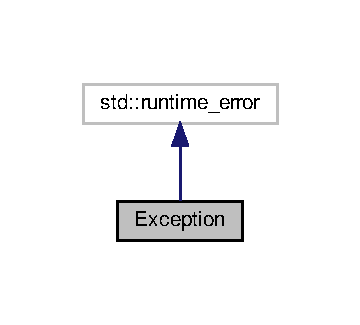
\includegraphics[width=173pt]{classException__inherit__graph}
\end{center}
\end{figure}


Collaboration diagram for Exception\+:\nopagebreak
\begin{figure}[H]
\begin{center}
\leavevmode
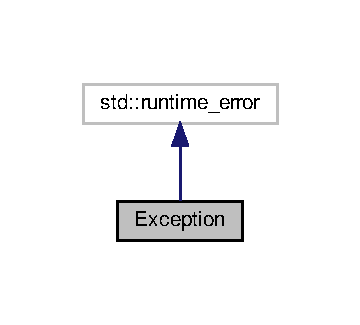
\includegraphics[width=173pt]{classException__coll__graph}
\end{center}
\end{figure}
\subsection*{Public Member Functions}
\begin{DoxyCompactItemize}
\item 
\hyperlink{classException_a53bf3b11d41090b81619796fc3a44b2c}{Exception} (const std\+::string \&message, const char $\ast$file, unsigned int line)
\item 
\mbox{\Hypertarget{classException_ae7ba8334eb35e001b4b0c6df9339c0dc}\label{classException_ae7ba8334eb35e001b4b0c6df9339c0dc}} 
const char $\ast$ \hyperlink{classException_ae7ba8334eb35e001b4b0c6df9339c0dc}{what} () const noexcept override
\begin{DoxyCompactList}\small\item\em Return a C-\/style string containing information about the error. \end{DoxyCompactList}\end{DoxyCompactItemize}


\subsection{Detailed Description}
Custom \hyperlink{classException}{Exception} class. Can be nested to have an error backtrace. 

\subsection{Constructor \& Destructor Documentation}
\mbox{\Hypertarget{classException_a53bf3b11d41090b81619796fc3a44b2c}\label{classException_a53bf3b11d41090b81619796fc3a44b2c}} 
\index{Exception@{Exception}!Exception@{Exception}}
\index{Exception@{Exception}!Exception@{Exception}}
\subsubsection{\texorpdfstring{Exception()}{Exception()}}
{\footnotesize\ttfamily Exception\+::\+Exception (\begin{DoxyParamCaption}\item[{const std\+::string \&}]{message,  }\item[{const char $\ast$}]{file,  }\item[{unsigned int}]{line }\end{DoxyParamCaption})\hspace{0.3cm}{\ttfamily [inline]}}

Builds an \hyperlink{classException}{Exception}. 
\begin{DoxyParams}{Parameters}
{\em message} & \mbox{[}in\mbox{]} The error message \\
\hline
{\em file} & \mbox{[}in\mbox{]} The file containing the error \\
\hline
{\em line} & \mbox{[}in\mbox{]} The line containing the error \\
\hline
\end{DoxyParams}


The documentation for this class was generated from the following file\+:\begin{DoxyCompactItemize}
\item 
/home/serdok/\+Projects/\+Game/src/hpp/Exceptions.\+hpp\end{DoxyCompactItemize}

\hypertarget{classGame}{}\section{Game Class Reference}
\label{classGame}\index{Game@{Game}}


\hyperlink{classGame}{Game} class.  




{\ttfamily \#include $<$Game.\+hpp$>$}

\subsection*{Public Member Functions}
\begin{DoxyCompactItemize}
\item 
\mbox{\Hypertarget{classGame_ad59df6562a58a614fda24622d3715b65}\label{classGame_ad59df6562a58a614fda24622d3715b65}} 
\hyperlink{classGame_ad59df6562a58a614fda24622d3715b65}{Game} ()
\begin{DoxyCompactList}\small\item\em Initialize game graphics engine. \end{DoxyCompactList}\item 
void \hyperlink{classGame_aa3ad98174079ae07b15cd6d29a04edc3}{Init} (const std\+::string \&title=std\+::string(), int width=800, int height=600, bool fullscreen=false)
\item 
\mbox{\Hypertarget{classGame_a96341ca5b54d90adc3ecb3bf0bcd2312}\label{classGame_a96341ca5b54d90adc3ecb3bf0bcd2312}} 
void \hyperlink{classGame_a96341ca5b54d90adc3ecb3bf0bcd2312}{Run} ()
\begin{DoxyCompactList}\small\item\em Run the game. Must be called after \hyperlink{classGame_aa3ad98174079ae07b15cd6d29a04edc3}{Init()}. \end{DoxyCompactList}\end{DoxyCompactItemize}
\subsection*{Static Public Member Functions}
\begin{DoxyCompactItemize}
\item 
\mbox{\Hypertarget{classGame_aa626467d3a202d2eca952c972fd2e0bf}\label{classGame_aa626467d3a202d2eca952c972fd2e0bf}} 
static \hyperlink{structSDL__WindowInfo}{S\+D\+L\+\_\+\+Window\+Info} \hyperlink{classGame_aa626467d3a202d2eca952c972fd2e0bf}{Get\+Window\+Info} ()
\begin{DoxyCompactList}\small\item\em Getter for the window info. \end{DoxyCompactList}\item 
\mbox{\Hypertarget{classGame_a258a5c5dc8fcb42562ce22338f355e7d}\label{classGame_a258a5c5dc8fcb42562ce22338f355e7d}} 
static S\+D\+L\+\_\+\+Renderer $\ast$ \hyperlink{classGame_a258a5c5dc8fcb42562ce22338f355e7d}{Get\+Renderer} ()
\begin{DoxyCompactList}\small\item\em Getter for the renderer. \end{DoxyCompactList}\item 
\mbox{\Hypertarget{classGame_a40692522c413451781d0fa2ecf7ca91a}\label{classGame_a40692522c413451781d0fa2ecf7ca91a}} 
static S\+D\+L\+\_\+\+Renderer\+Info \hyperlink{classGame_a40692522c413451781d0fa2ecf7ca91a}{Get\+Renderer\+Info} ()
\begin{DoxyCompactList}\small\item\em Getter for the renderer info. \end{DoxyCompactList}\item 
\mbox{\Hypertarget{classGame_a7ea06dbc77dccebed1e9a7acd4966d7b}\label{classGame_a7ea06dbc77dccebed1e9a7acd4966d7b}} 
static S\+D\+L\+\_\+\+Event \hyperlink{classGame_a7ea06dbc77dccebed1e9a7acd4966d7b}{Get\+Events} ()
\begin{DoxyCompactList}\small\item\em Getter for the game events. \end{DoxyCompactList}\item 
\mbox{\Hypertarget{classGame_a4c2d2d2e8b4477c6addc2741047e399b}\label{classGame_a4c2d2d2e8b4477c6addc2741047e399b}} 
static S\+D\+L\+\_\+\+Rect \hyperlink{classGame_a4c2d2d2e8b4477c6addc2741047e399b}{Get\+Camera} ()
\begin{DoxyCompactList}\small\item\em Getter for the game camera. \end{DoxyCompactList}\end{DoxyCompactItemize}


\subsection{Detailed Description}
\hyperlink{classGame}{Game} class. 

\subsection{Member Function Documentation}
\mbox{\Hypertarget{classGame_aa3ad98174079ae07b15cd6d29a04edc3}\label{classGame_aa3ad98174079ae07b15cd6d29a04edc3}} 
\index{Game@{Game}!Init@{Init}}
\index{Init@{Init}!Game@{Game}}
\subsubsection{\texorpdfstring{Init()}{Init()}}
{\footnotesize\ttfamily void Game\+::\+Init (\begin{DoxyParamCaption}\item[{const std\+::string \&}]{title = {\ttfamily std\+:\+:string()},  }\item[{int}]{width = {\ttfamily 800},  }\item[{int}]{height = {\ttfamily 600},  }\item[{bool}]{fullscreen = {\ttfamily false} }\end{DoxyParamCaption})}

Initialize the game components 
\begin{DoxyParams}{Parameters}
{\em title} & \mbox{[}in\mbox{]} The window title \\
\hline
{\em width} & \mbox{[}in\mbox{]} The window width \\
\hline
{\em height} & \mbox{[}in\mbox{]} The window height \\
\hline
{\em fullscreen} & \mbox{[}in\mbox{]} If the game should run on fullscreen \\
\hline
\end{DoxyParams}


The documentation for this class was generated from the following files\+:\begin{DoxyCompactItemize}
\item 
/home/serdok/\+Universite/\+L2/\+L\+I\+F\+A\+P4/\+Game/src/hpp/Game.\+hpp\item 
/home/serdok/\+Universite/\+L2/\+L\+I\+F\+A\+P4/\+Game/src/cpp/Game.\+cpp\end{DoxyCompactItemize}

\hypertarget{structSDL__WindowInfo}{}\section{S\+D\+L\+\_\+\+Window\+Info Struct Reference}
\label{structSDL__WindowInfo}\index{S\+D\+L\+\_\+\+Window\+Info@{S\+D\+L\+\_\+\+Window\+Info}}


Structure containing useful window info.  




{\ttfamily \#include $<$Game.\+hpp$>$}

\subsection*{Public Attributes}
\begin{DoxyCompactItemize}
\item 
\mbox{\Hypertarget{structSDL__WindowInfo_acd6a7d7cba722414292a594a3d48445c}\label{structSDL__WindowInfo_acd6a7d7cba722414292a594a3d48445c}} 
std\+::string \hyperlink{structSDL__WindowInfo_acd6a7d7cba722414292a594a3d48445c}{title}
\begin{DoxyCompactList}\small\item\em Title of the window. \end{DoxyCompactList}\item 
\mbox{\Hypertarget{structSDL__WindowInfo_ab70b2d2424fe9f5e2f4e86c0e2be771a}\label{structSDL__WindowInfo_ab70b2d2424fe9f5e2f4e86c0e2be771a}} 
int \hyperlink{structSDL__WindowInfo_ab70b2d2424fe9f5e2f4e86c0e2be771a}{x}
\begin{DoxyCompactList}\small\item\em Position of the window. \end{DoxyCompactList}\item 
\mbox{\Hypertarget{structSDL__WindowInfo_a8734912a3d6df22e9a7a31ae5eb291a2}\label{structSDL__WindowInfo_a8734912a3d6df22e9a7a31ae5eb291a2}} 
int \hyperlink{structSDL__WindowInfo_a8734912a3d6df22e9a7a31ae5eb291a2}{y}
\begin{DoxyCompactList}\small\item\em Position of the window. \end{DoxyCompactList}\item 
\mbox{\Hypertarget{structSDL__WindowInfo_aa1e54155607b67024630859f2126c88b}\label{structSDL__WindowInfo_aa1e54155607b67024630859f2126c88b}} 
int \hyperlink{structSDL__WindowInfo_aa1e54155607b67024630859f2126c88b}{width}
\begin{DoxyCompactList}\small\item\em Size of the window. \end{DoxyCompactList}\item 
\mbox{\Hypertarget{structSDL__WindowInfo_abb321b367d4221fac50b8d10f03283c2}\label{structSDL__WindowInfo_abb321b367d4221fac50b8d10f03283c2}} 
int \hyperlink{structSDL__WindowInfo_abb321b367d4221fac50b8d10f03283c2}{height}
\begin{DoxyCompactList}\small\item\em Size of the window. \end{DoxyCompactList}\item 
\mbox{\Hypertarget{structSDL__WindowInfo_a54b7260c4504d9cc2dbe3a910811171c}\label{structSDL__WindowInfo_a54b7260c4504d9cc2dbe3a910811171c}} 
Uint32 \hyperlink{structSDL__WindowInfo_a54b7260c4504d9cc2dbe3a910811171c}{flags}
\begin{DoxyCompactList}\small\item\em Flags of the window. \end{DoxyCompactList}\end{DoxyCompactItemize}


\subsection{Detailed Description}
Structure containing useful window info. 

The documentation for this struct was generated from the following file\+:\begin{DoxyCompactItemize}
\item 
/home/serdok/\+Projects/\+Game/src/hpp/Game.\+hpp\end{DoxyCompactItemize}

%--- End generated contents ---

% Index
\backmatter
\newpage
\phantomsection
\clearemptydoublepage
\addcontentsline{toc}{chapter}{Index}
\printindex

\end{document}
